\documentclass[a4paper,12pt]{article} % тип документа

%  Русский язык
\usepackage[T2A]{fontenc}			% кодировка
\usepackage[utf8]{inputenc}			% кодировка исходного текста
\usepackage[english,russian]{babel}	% локализация и переносы

\usepackage{graphicx}               % импорт изображений
\usepackage{wrapfig}                % обтекаемые изображения
\graphicspath{{pictures/}}          % обращение к подкаталогу с изображениями
\usepackage[14pt]{extsizes}         % для того чтобы задать нестандартный 14-ый размер шрифта
\usepackage{amsfonts}               % буквы с двойными штрихами
\usepackage[warn]{mathtext}         % русский язык в формулах
\usepackage{indentfirst}            % indent first
\usepackage[margin = 25mm]{geometry}% отступы полей
\usepackage{amsmath}                % можно выводить фигурные скобочки -- делать системы уравнений
\usepackage[table,xcdraw]{xcolor}   % таблицы
\usepackage{amsmath,amsfonts,amssymb,amsthm,mathtools} % Математика
\usepackage{wasysym}                % ???
\usepackage{upgreek}                % ???  
\usepackage{caption}
\captionsetup{labelsep=period}
\usepackage{gensymb} % degree symbol


\begin{document}
	
	
	\begin{center}
		
		
		\textbf{НАЦИОНАЛЬНЫЙ ИССЛЕДОВАТЕЛЬСКИЙ УНИВЕРСИТЕТ \\ <<МОСКОВСКИЙ ФИЗИКО-ТЕХНИЧЕСКИЙ ИНСТИТУТ>>}
		\vspace{13ex}
		
		\textbf{Лабораторная работа 3.2.3\\ <<Резонанс токов в параллельном контуре>>}
		\vspace{40ex}
		
		\normalsize{Овсянников Михаил Александрович \\ студент группы Б01-001\\ 2 курс ФРКТ\\}
	\end{center}
	
	\vfill 
	
	\begin{center}
		г. Долгопрудный\\ 
		2021 г.
	\end{center}
	
	
	\thispagestyle{empty} % выключаем отображение номера для этой страницы
	\newpage
	
	\setcounter{page}{12}
	
	\textbf{Цель работы:} исследование резонанса токов в параллельном колебательном контуре с изменяемой ёмкостью, включающее получение амплитудно-частотных характеристик, а также определение основных параметров контура.
	
	
	\textbf{В работе используются:} генератор сигналов, источник тока, нагруженный на параллельный колебательный контур с переменной ёмкостью, двулучевой осциллограф, цифровые вольтметры.
	
	
	Схема экспериментального стенда для изучения резонанса токов в параллельном колебательном контуре показана на рисунке 1. Синусоидальный сигнал от генератора GFG-8255A поступает на вход источника тока, собранного на операционном усилителе ОУ с полевым транзистором ПТ, питание которых осуществляется встроенным блоком-выпрямителем от сети переменного тока 220 вольт. Источник тока, обладающий по определению бесконечным внутренним сопротивлением, фактически обеспечивает постоянство амплитуды тока $I$ на меняющейся по величине нагрузке – параллельном контуре. у. Источник тока, колебательный контур и блок питания заключены в отдельный корпус с названием «Резонанс токов» на верхней крышке, отмеченный на рисунке штриховой линией.

	
	На корпусе имеются коаксиальные разъёмы «Вход», «U$_1$» и «U$_2$», а также переключатель магазина ёмкостей $C_n$ с указателем номера $n = 1, 2, … 7$. Напряжение $E =E_0\cos(\omega t + \varphi_0)$ поступает на вход «+» операционного усилителя от генератора через согласующую RC-цепочку. Это же напряжение через разъём «U$_1$» подаётся одновременно на канал 1 осциллографа GOS-620 и вход 1-го цифрового вольтметра GDM-8245.
	\begin{figure}[h!]
		\centering
		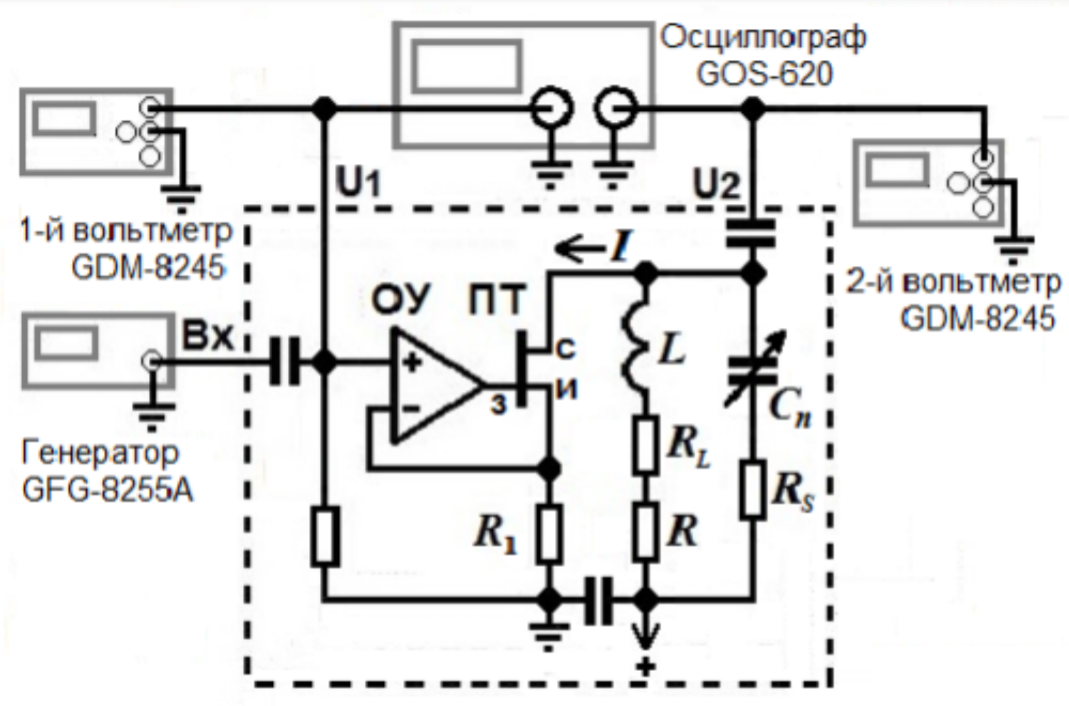
\includegraphics[scale=0.6]{Pictures/Установка.png}
		\caption*{Рис. 1. Схема экспериментального стенда}
	\end{figure}

\vspace{7mm}
Выпишем необходимые формулы.

Собственная резонансная частота:

\begin{equation*}
	f_r = \frac{1}{2\pi\sqrt{LC_L}}
\end{equation*}

Эквивалентное последовательное сопротивление:

\begin{equation*}
	R_S = \frac{1}{\omega C}\tg(\delta)
\end{equation*}

Ёмкостный и индуктивный импедансы соответственно:

\begin{equation*}
	Z_C = R_S - \frac{i}{\omega C}, \hspace{35mm} Z_L = R + R_L + i\omega L
\end{equation*}


Амплитуда тока на конденсаторе:

\begin{equation*}
	I_C = QI_0\frac{\omega}{\omega_0}\frac{e^{i\varphi_C}}{\sqrt{1 + (\tau\Delta\omega)^2}}, \hspace{25mm} \varphi_C = \frac{\pi}{2} - \frac{R+R_L}{\rho} - \arctg(\tau\Delta\omega).
\end{equation*}

Амплитуда тока на катушке:

\begin{equation*}
	I_C = QI_0\frac{\omega_0}{\omega}\frac{e^{i\varphi_L}}{\sqrt{1 + (\tau\Delta\omega)^2}}, \hspace{25mm} \varphi_L = -\frac{\pi}{2} +\delta - \arctg(\tau\Delta\omega).
\end{equation*}

Амплитуда напряжения:

\begin{equation*}
	I_C = Q\rho I_0\frac{e^{i\varphi_U}}{\sqrt{1 + (\tau\Delta\omega)^2}}, \hspace{25mm} \varphi_U = -\frac{\omega_0}{\omega}\frac{R+R_L}{\rho} + \delta - \arctg(\tau\Delta\omega).
\end{equation*}
		
\newpage

Выставим входное напряжение $U_{\text{вх}} = 100$ мВ.


Для контуров с пятью различными ёмкостями измерим резонансные частоты и $f_{\text{р}}$ напряжения $U(f_{\text{р}})$.


\begin{table}[h!]
	\centering
	\begin{tabular}{|c|c|c|c|c|c|}
		\hline
		$U_0$, мВ & $U_C$, мВ & $C$, нФ & \begin{tabular}[c]{@{}c@{}}$f_{\text{р}}$, кГц \\ (Лиссажу)\end{tabular} & \begin{tabular}[c]{@{}c@{}}$f_{\text{р}}$, кГц \\ (Развертка)\end{tabular} & $T = 2\pi \sqrt{LC}$, мкс \\ \hline
		100       & 286       & 47,9    & 23,77                                                                    & 23,56                                                                      & 42                       \\ \hline
		100       & 230       & 57,4    & 21,50                                                                    & 21,25                                                                      & 47                       \\ \hline
		100       & 192       & 66,7    & 19,98                                                                    & 19,72                                                                      & 51                       \\ \hline
		100       & 152       & 82,1    & 18,07                                                                    & 17,74                                                                      & 56                       \\ \hline
		100       & 124       & 99,6    & 16,45                                                                    & 16,19                                                                      & 62                       \\ \hline
	\end{tabular}
\end{table}
		
Построим график $\frac{T^2}{4\pi ^2}(C)$ и по наклону найдем индуктивность $L$.

\begin{table}[h!]
	\centering
	\begin{tabular}{|c|c|c|c|c|c|}
		\hline
		$C$, нФ                        & 47,9 & 57,4 & 66,7 & 82,1 & 99,6 \\ \hline
		$\frac{T^2}{4\pi ^2}$, мкс$^2$ & 45 & 56 & 66 & 79 & 92 \\ \hline
	\end{tabular}
\end{table}

\begin{figure}[h!]
	\centering
	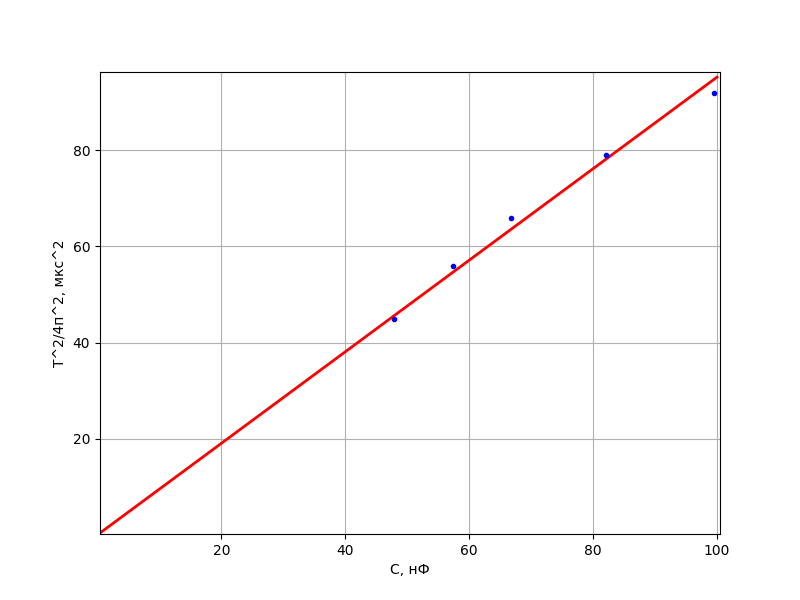
\includegraphics[scale=0.80]{Pictures/T(C).png}
\end{figure}
		
Используя МНК, получаем:

$L = 0,95$ мГн

$\sigma_L = 0,01$ мГн.
\newpage

Для контуров с двумя разными ёмкостями снимем амплитудно-частотные характеристики.

1) $C = 47,9$ нФ. $f_{\text{р}} = 23,56$ кГц.

\begin{table}[h!]
	\centering
	\begin{tabular}{|c|c|c|c|}
		\hline
		$U_0$, мВ & $U_C$, мВ & $A = \sqrt{2}U_C$, мВ & $f$, кГц \\ \hline
		100       & 42        & 59,4                  & 14,15   \\ \hline
		100       & 44        & 62,2                  & 16,45   \\ \hline
		100       & 52        & 73,5                  & 18,83   \\ \hline
		100       & 82        & 116,0                 & 21,22   \\ \hline
		100       & 131       & 185,3                 & 22,35   \\ \hline
		100       & 207       & 292,7                 & 23,00   \\ \hline
		100       & 286       & 404,5                 & 23,56   \\ \hline
		100       & 227       & 321,0                 & 24,05   \\ \hline
		100       & 120       & 169,7                 & 24,78   \\ \hline
		100       & 58        & 82,0                  & 25,97   \\ \hline
		100       & 26        & 36,8                  & 28,21   \\ \hline
		100       & 10        & 14,1                  & 31,04   \\ \hline
	\end{tabular}
\end{table}

Получаем следующий график:

\begin{figure}[h!]
	\centering
	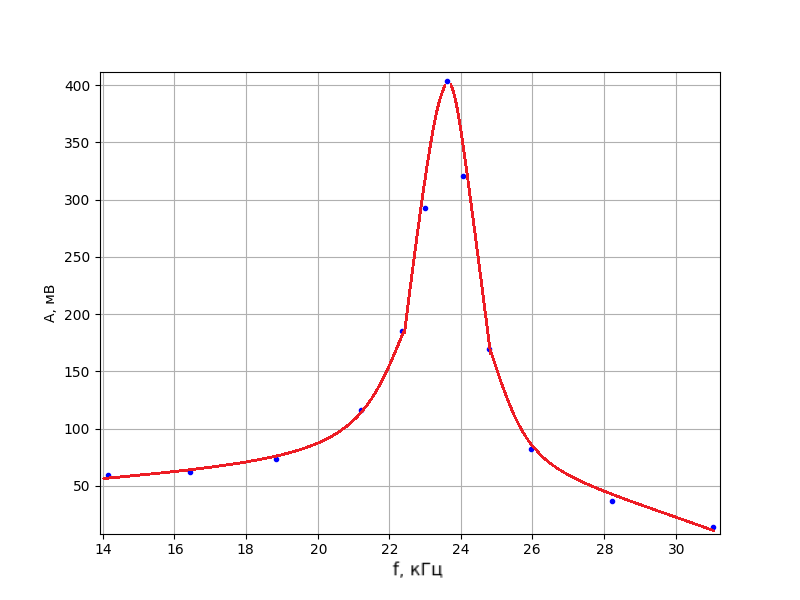
\includegraphics[scale=0.85]{Pictures/Рез1.png}
\end{figure}
\newpage
Из него найдем добротность $Q = \frac{f_{\text{р}}}{\Delta f} = \frac{23,56}{1,29} \approx 18,3$ ($\Delta f$ измеряется на высоте $\frac{A_{max}}{\sqrt{2}}$).

\begin{figure}[h!]
	\centering
	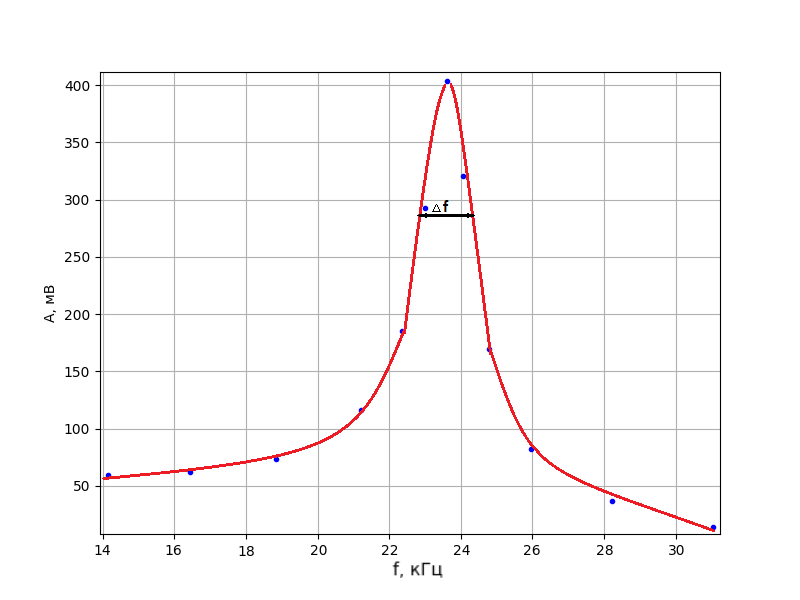
\includegraphics[scale=0.85]{Pictures/Рез1Добр.png}
\end{figure}

2) $C = 82,1$ нФ. $f_{\text{р}} = 178,0$ Гц.

\begin{table}[h!]
	\centering
	\begin{tabular}{|c|c|c|c|}
		\hline
		$U_0$, мВ & $U_C$, мВ & $A = \sqrt{2}U_C$, мВ & $f$, кГц \\ \hline
		100       & 47,9      & 67,7                  & 10,68   \\ \hline
		100       & 47,1      & 66,6                  & 12,42   \\ \hline
		100       & 51,6      & 73,0                  & 14,20   \\ \hline
		100       & 71,6      & 101,3                 & 16,00   \\ \hline
		100       & 99,8      & 141,1                 & 17,80   \\ \hline
		100       & 36,4      & 51,5                  & 19,56   \\ \hline
		100       & 9,7       & 13,7                  & 21,30   \\ \hline
	\end{tabular}
\end{table}

График:
\newpage

\begin{figure}[h!]
	\centering
	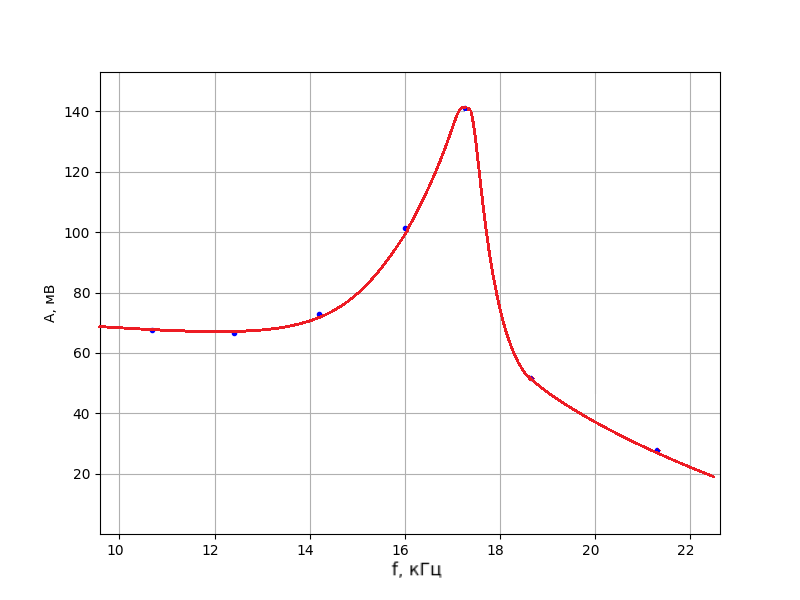
\includegraphics[scale=0.85]{Pictures/Рез2.png}
\end{figure}

Найдем добротность $Q = \frac{f_{\text{р}}}{\Delta f} \approx 12.1$

Как видим, $\frac{Q_1}{Q_2} = 1.51 \approx \sqrt{2}$.

\begin{figure}[h!]
	\centering
	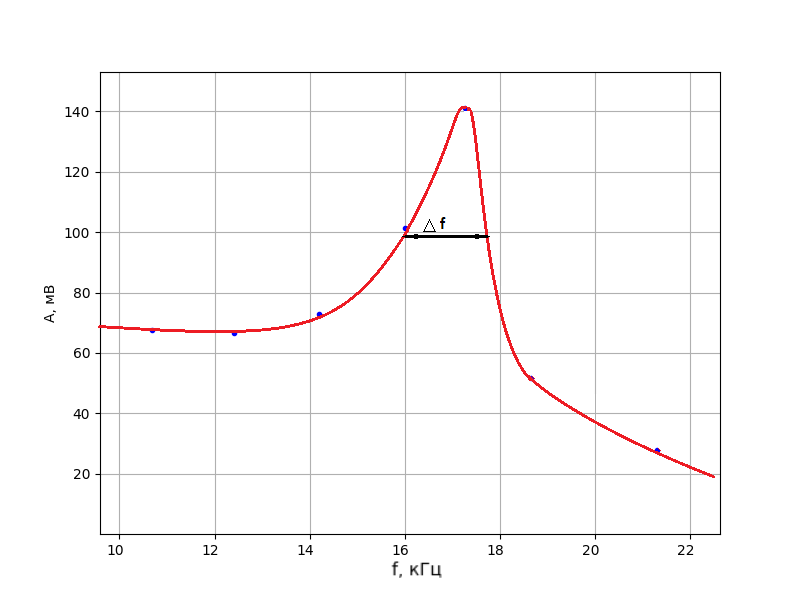
\includegraphics[scale=0.85]{Pictures/Рез2Добр.png}
\end{figure}
\newpage
\begin{figure}[h!]
	\centering
	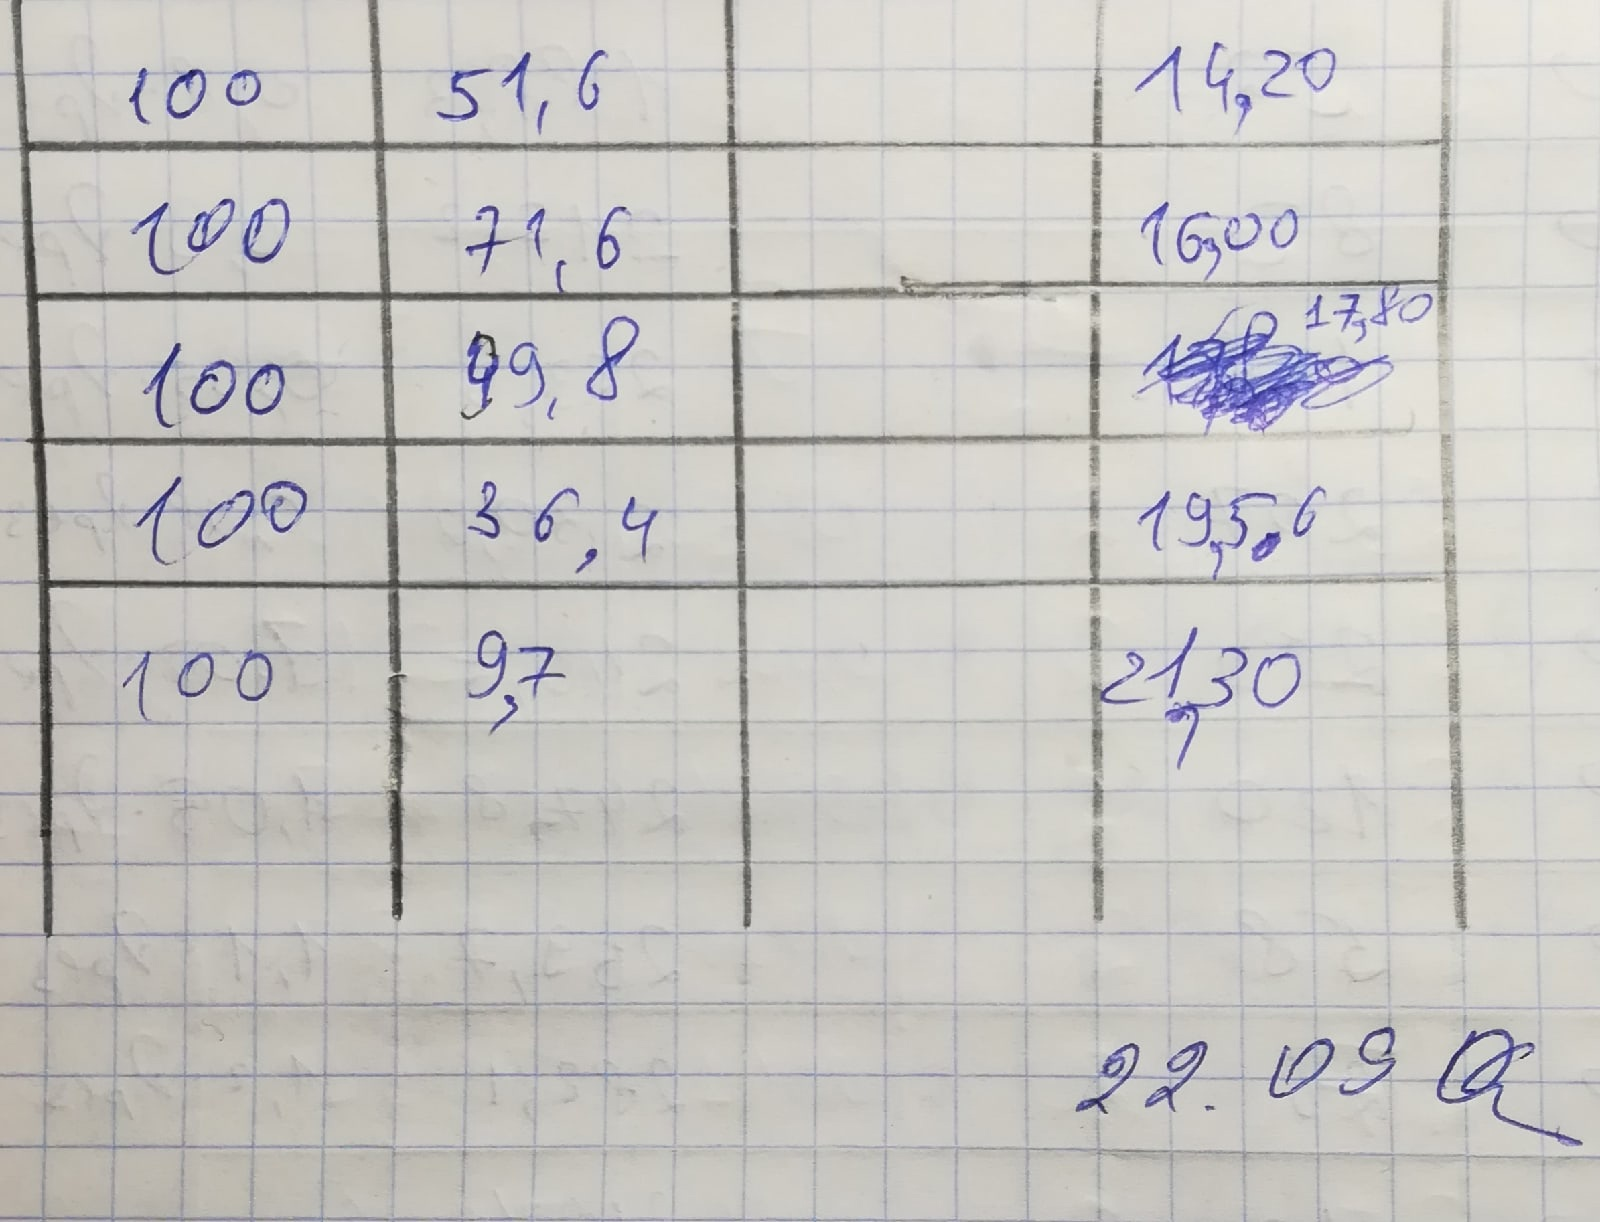
\includegraphics[scale=0.25]{Pictures/Табл.jpg}
\end{figure}

\textbf{Вывод:} в работе было проведено исследование резонанса токов в параллельном колебательном контуре с изменяемой ёмкостью. Были получены амплитудно-частотные характеристики, а также определены основные параметры контура $L = (0,95 \pm 0,01)$ мГн. Все ошибки связаны с неточностью измерений и несовершенной техникой измерений.

\end{document}









